\section{Capítulo 9 -- Recursão e backtracking}

No Capítulo 6, as funções chamavam outras funções. Nada impede que uma função chame \textbf{a si mesma}, e essa ideia, a \textbf{recursão}, é uma das mais poderosas da programação. Muitos problemas são naturalmente definidos em termos de versões menores deles mesmos: o fatorial de 5 é 5 vezes o fatorial de 4; uma pasta contém arquivos e outras pastas; para mover uma pilha de discos, move-se uma pilha menor. Neste capítulo você vai aprender a escrever funções recursivas, a entender o que acontece na pilha de chamadas a cada uma delas, a reconhecer quando a recursão é uma boa escolha e quando é um desperdício, e a usá-la na técnica de \textbf{backtracking}, que explora sistematicamente todas as possibilidades de um problema.

\subsection{9.1 Uma função que chama a si mesma}

O fatorial de um número $n$, escrito $n!$, é o produto de todos os inteiros de 1 até $n$: $4! = 4 \times 3 \times 2 \times 1 = 24$. No Capítulo 5, ele seria calculado com um laço. Mas repare que $4! = 4 \times 3!$, e em geral $n! = n \times (n-1)!$. Essa é uma \textbf{definição recursiva}: o fatorial é definido usando o próprio fatorial, de um número menor. Para que ela não continue para sempre, é preciso um ponto de parada: $1! = 1$ (e, por convenção, $0! = 1$).

Toda função recursiva tem essas duas partes:

\begin{itemize}
  \item o \textbf{caso base}, um caso simples o bastante para ser respondido diretamente, sem recursão;
  \item o \textbf{caso recursivo}, que resolve o problema usando a resposta de um problema \textbf{menor} do mesmo tipo, cada vez mais perto do caso base.
\end{itemize}

\begin{codigo}
\begin{Verbatim}[breaklines=true, breaksymbolleft={}, fontsize=\footnotesize]
#include <iostream>
using namespace std;

long long fatorial(int n) {
    if (n <= 1) return 1;              // caso base
    return n * fatorial(n - 1);        // caso recursivo
}

int main() {
    int n;
    cout << "n (0 a 20): ";
    cin >> n;
    if (n < 0 || n > 20) {
        cout << "Fora da faixa." << endl;   // 21! não cabe
        return 0;
    }
    cout << n << "! = " << fatorial(n) << endl;
    return 0;
}
// 4 -> 4! = 24        20 -> 20! = 2432902008176640000
\end{Verbatim}
\end{codigo}

O tipo \texttt{long long} guarda inteiros de até cerca de $9{,}2 \times 10^{18}$. Como o fatorial cresce muito depressa, $20!$ é o maior que cabe nele, e por isso o programa recusa valores maiores.

O Portugol também aceita funções recursivas, com a mesma estrutura:

\begin{codigo}
\begin{Verbatim}[breaklines=true, breaksymbolleft={}, fontsize=\footnotesize]
algoritmo "FatorialRecursivo"
var
   n: inteiro

funcao fatorial(k: inteiro): inteiro
inicio
   se k <= 1 entao
      retorne 1
   senao
      retorne k * fatorial(k - 1)
   fimse
fimfuncao

inicio
   escreva("n: ")
   leia(n)
   escreval(n, "! = ", fatorial(n))
fimalgoritmo
\end{Verbatim}
\end{codigo}

\subsection{9.2 O que acontece na pilha de chamadas}

Uma chamada recursiva funciona exatamente como qualquer outra chamada (Seção 6.4): ela ganha seu próprio registro de ativação na pilha, com seu próprio \texttt{n}. A chamada \texttt{fatorial(4)} não termina enquanto não recebe a resposta de \texttt{fatorial(3)}, que espera \texttt{fatorial(2)}, que espera \texttt{fatorial(1)}. Por um momento, há quatro registros empilhados, cada um com um \texttt{n} diferente. Só então as respostas voltam, na ordem inversa, e cada chamada completa sua multiplicação:

\begin{center}
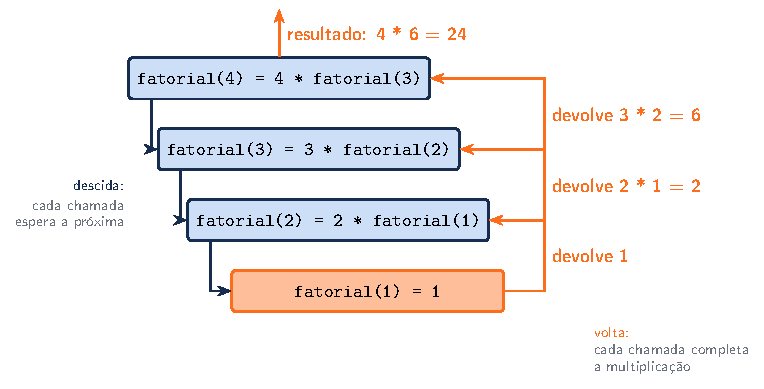
\includegraphics[width=0.85\linewidth,keepaspectratio]{imagens/capitulo-09_fatorial.pdf}
\end{center}

Esse ``ir e voltar'' tem duas consequências práticas. Primeiro, o trabalho de cada chamada se divide em duas partes: o que ela faz \textbf{antes} da chamada recursiva (na descida) e o que ela faz \textbf{depois} (na volta). No fatorial, a multiplicação acontece na volta. Segundo, a pilha tem tamanho limitado, normalmente de alguns megabytes. Uma recursão muito profunda, ou uma sem caso base, enche a pilha, e o programa é encerrado com um erro de \textbf{estouro de pilha} (\textit{stack overflow}):

\begin{codigo}
\begin{Verbatim}[breaklines=true, breaksymbolleft={}, fontsize=\footnotesize]
// erro: sem caso base, a recursão nunca termina
long long fatorial(int n) {
    return n * fatorial(n - 1);   // 4, 3, 2, 1, 0, -1, -2...
}
\end{Verbatim}
\end{codigo}

O mesmo acontece quando o caso base existe, mas a recursão nunca o alcança: se o teste fosse \texttt{if (n == 1)}, a chamada \texttt{fatorial(-3)} desceria para $-4$, $-5$\ldots{} sem nunca passar pelo 1. É por isso que o programa usa \texttt{n <= 1}. Por isso a regra da Seção 9.1: cada chamada recursiva precisa ser com um problema \textbf{menor}, que caminhe na direção do caso base.

\subsection{9.3 Pensando recursivamente}

Para escrever uma função recursiva, não tente acompanhar mentalmente todas as chamadas. Faça três perguntas: qual é o caso mais simples, que eu sei responder direto? Como diminuo o problema? E, \textbf{supondo que a chamada recursiva já funciona} para o problema menor, como uso a resposta dela para resolver o problema inteiro? Esse ato de confiança é o coração do raciocínio recursivo. Veja como ele resolve quatro problemas diferentes:

\begin{codigo}
\begin{Verbatim}[breaklines=true, breaksymbolleft={}, fontsize=\footnotesize]
#include <iostream>
#include <string>
using namespace std;

// b elevado a e: b^0 = 1; b^e = b * b^(e-1)
long long potencia(long long b, int e) {
    if (e == 0) return 1;
    return b * potencia(b, e - 1);
}

// soma dos n primeiros elementos: a soma dos n-1 primeiros
// mais o último
int soma(const int v[], int n) {
    if (n == 0) return 0;              // vetor vazio
    return soma(v, n - 1) + v[n - 1];
}

// inverter: o resto invertido, seguido da primeira letra
string inverter(const string &s) {
    if (s.size() <= 1) return s;
    return inverter(s.substr(1)) + s[0];
}

// máximo divisor comum, pelo algoritmo de Euclides
int mdc(int a, int b) {
    if (b == 0) return a;
    return mdc(b, a % b);
}

int main() {
    int v[] = {4, 8, 15, 16, 23, 42};
    cout << potencia(2, 10) << endl;       // 1024
    cout << soma(v, 6) << endl;            // 108
    cout << inverter("recursão") << endl;  // cuidado: acento!
    cout << inverter("pilha") << endl;     // ahlip
    cout << mdc(48, 18) << endl;           // 6
    return 0;
}
\end{Verbatim}
\end{codigo}

O algoritmo de Euclides, com mais de dois mil anos, usa um fato da aritmética: o MDC de \texttt{a} e \texttt{b} é igual ao MDC de \texttt{b} e do resto de \texttt{a} por \texttt{b}. A sequência de chamadas para 48 e 18 é \texttt{mdc(48, 18)}, \texttt{mdc(18, 12)}, \texttt{mdc(12, 6)} e \texttt{mdc(6, 0)}, que devolve 6. O \texttt{inverter("recursão")} foi incluído de propósito, para lembrar a Seção 8.7: ele inverte os bytes, e o \texttt{ã}, que ocupa dois, sai embaralhado.

\subsection{9.4 Quando a recursão desperdiça: Fibonacci}

A sequência de Fibonacci começa com 0 e 1, e cada termo seguinte é a soma dos dois anteriores: 0, 1, 1, 2, 3, 5, 8, 13, 21\ldots{} A definição é recursiva, e a função sai quase igual a ela: \texttt{fib(n) = fib(n - 1) + fib(n - 2)}, com \texttt{fib(0) = 0} e \texttt{fib(1) = 1} como casos base. Mas há um problema escondido. Cada chamada faz \textbf{duas} chamadas recursivas, e elas repetem o mesmo trabalho:

\begin{center}
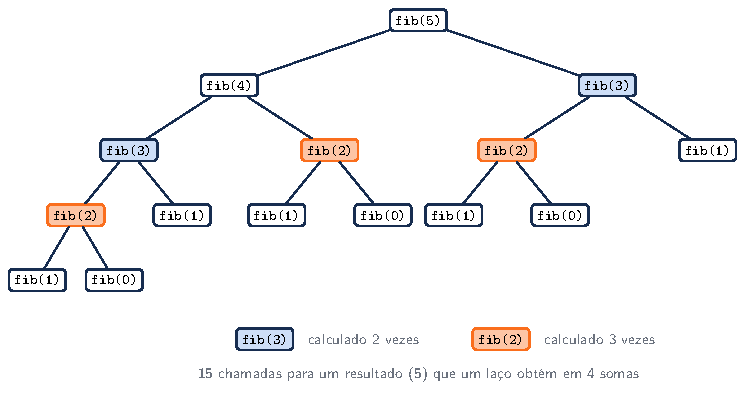
\includegraphics[width=0.9\linewidth,keepaspectratio]{imagens/capitulo-09_fibonacci.pdf}
\end{center}

Só para calcular \texttt{fib(5)}, o \texttt{fib(2)} é calculado três vezes. Para valores maiores, a repetição explode: o número de chamadas cresce quase tão depressa quanto a própria sequência. O programa abaixo conta as chamadas e compara com uma versão que guarda cada resultado já calculado em um vetor e o consulta antes de recalcular. Essa técnica se chama \textbf{memoização}.

\begin{codigo}
\begin{Verbatim}[breaklines=true, breaksymbolleft={}, fontsize=\footnotesize]
#include <iostream>
#include <vector>
using namespace std;

long long fib(int n, long long &chamadas) {
    chamadas++;
    if (n <= 1) return n;
    return fib(n - 1, chamadas) + fib(n - 2, chamadas);
}

long long fibMemo(int n, vector<long long> &memo) {
    if (n <= 1) return n;
    if (memo[n] != 0) return memo[n];        // já calculado
    memo[n] = fibMemo(n - 1, memo) + fibMemo(n - 2, memo);
    return memo[n];
}

int main() {
    for (int n = 10; n <= 30; n += 10) {
        long long chamadas = 0;
        long long f = fib(n, chamadas);
        cout << "fib(" << n << ") = " << f << ", "
             << chamadas << " chamadas" << endl;
    }
    vector<long long> memo(91, 0);
    cout << "fib(90) = " << fibMemo(90, memo) << endl;
    return 0;
}
// fib(10) = 55, 177 chamadas
// fib(20) = 6765, 21891 chamadas
// fib(30) = 832040, 2692537 chamadas
// fib(90) = 2880067194370816120
\end{Verbatim}
\end{codigo}

A versão simples precisa de quase 2,7 milhões de chamadas para \texttt{fib(30)}, e de mais de 330 milhões para \texttt{fib(40)}. Para \texttt{fib(90)}, ela levaria séculos. A versão com memoização calcula cada termo uma única vez e chega a \texttt{fib(90)} com menos de 200 chamadas. Um simples laço, que vai somando os dois últimos termos, resolveria com a mesma rapidez. A lição: uma definição recursiva elegante não é, necessariamente, um bom algoritmo.

\subsection{9.5 Recursão ou laço?}

Todo laço pode ser escrito como recursão, e toda recursão pode ser escrita com laços (às vezes com a ajuda de uma pilha explícita). A escolha é sobre clareza e custo:

\begin{center}
\begin{tabular}{@{}p{0.44\linewidth}p{0.44\linewidth}@{}}
\toprule
\rowcolor{headergray}
\tblheader{Prefira o laço quando} & \tblheader{Prefira a recursão quando} \\
\midrule
o problema é uma sequência simples de passos, como somar, contar, fatorial & o problema se divide em subproblemas do mesmo tipo, como pastas, árvores, Torres de Hanói \\
\rowcolor{rowgray} a profundidade pode ser muito grande (milhares de níveis) & a profundidade é pequena, ou cresce devagar \\
a versão recursiva repete trabalho, como no Fibonacci & é preciso explorar possibilidades e voltar atrás (backtracking) \\
\bottomrule
\end{tabular}
\end{center}

Cada chamada recursiva custa um pouco mais que uma volta de laço, porque precisa criar e destruir um registro na pilha. Nos exemplos simples da Seção 9.3, o laço seria um pouco mais eficiente. Nos problemas das próximas seções, a recursão é tão mais clara que a versão com laços quase ninguém escreveria.

\subsection{9.6 As Torres de Hanói}

O quebra-cabeça das Torres de Hanói tem três pinos e uma pilha de discos de tamanhos diferentes, todos no primeiro pino, do maior (embaixo) para o menor. O objetivo é levar a pilha inteira para o terceiro pino, movendo \textbf{um disco por vez} e \textbf{nunca} colocando um disco sobre outro menor.

\begin{center}
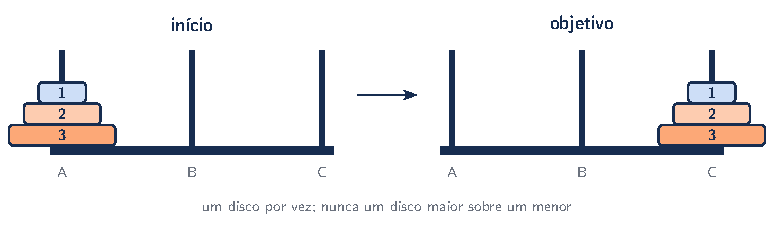
\includegraphics[width=0.9\linewidth,keepaspectratio]{imagens/capitulo-09_hanoi.pdf}
\end{center}

Com laços, é difícil até começar. Com o raciocínio recursivo, a solução cabe em três frases. Para mover $n$ discos de A para C, usando B como apoio:

\begin{enumerate}
  \item mova os $n - 1$ discos de cima de A para B (usando C como apoio);
  \item mova o maior disco, que ficou sozinho, de A para C;
  \item mova os $n - 1$ discos de B para C (usando A como apoio).
\end{enumerate}

Os passos 1 e 3 são o mesmo problema, com um disco a menos: é a ``confiança'' da Seção 9.3. O caso base é mover zero discos, que não exige nada.

\begin{codigo}
\begin{Verbatim}[breaklines=true, breaksymbolleft={}, fontsize=\footnotesize]
#include <iostream>
using namespace std;

void hanoi(int n, char origem, char destino, char apoio,
           int &movimentos) {
    if (n == 0) return;                        // caso base
    hanoi(n - 1, origem, apoio, destino, movimentos);
    movimentos++;
    cout << movimentos << ": disco " << n << " de " << origem
         << " para " << destino << endl;
    hanoi(n - 1, apoio, destino, origem, movimentos);
}

int main() {
    int movimentos = 0;
    hanoi(3, 'A', 'C', 'B', movimentos);
    cout << movimentos << " movimentos" << endl;   // 7
    return 0;
}
// 1: disco 1 de A para C     5: disco 1 de B para A
// 2: disco 2 de A para B     6: disco 2 de B para C
// 3: disco 1 de C para B     7: disco 1 de A para C
// 4: disco 3 de A para C
\end{Verbatim}
\end{codigo}

Cada disco a mais dobra o trabalho e acrescenta um movimento: com $n$ discos, são $2^n - 1$ movimentos. Com 3 discos, 7; com 10, 1.023; com 64 discos, como na lenda que deu origem ao quebra-cabeça, mais de 18 quintilhões, o que levaria mais de 500 bilhões de anos a um movimento por segundo.

\subsection{9.7 Backtracking: tentar, avançar e voltar atrás}

Muitos problemas pedem que se encontre uma combinação de escolhas que satisfaça certas regras: preencher um sudoku, montar um horário sem conflitos, encontrar a saída de um labirinto. O \textbf{backtracking} (``voltar atrás'') resolve esse tipo de problema fazendo uma escolha de cada vez:

\begin{enumerate}
  \item se todas as escolhas já foram feitas, encontrou-se uma solução;
  \item senão, para cada opção possível da próxima escolha: se ela não viola as regras, faça-a, continue recursivamente com as escolhas seguintes e, ao voltar, \textbf{desfaça} a escolha para tentar a próxima opção.
\end{enumerate}

A recursão cuida de lembrar onde se estava: quando uma tentativa leva a um beco sem saída, a função simplesmente retorna, e a chamada anterior continua com sua próxima opção. Um exemplo simples é gerar todas as \textbf{permutações} de um texto, ou seja, todas as ordens possíveis de suas letras. A cada posição \texttt{k}, escolhe-se qual letra vai ocupá-la, trocando-a para lá; depois de permutar o resto, a troca é desfeita:

\begin{codigo}
\begin{Verbatim}[breaklines=true, breaksymbolleft={}, fontsize=\footnotesize]
#include <iostream>
#include <string>
using namespace std;

void permutar(string &s, int k) {
    if (k == int(s.size())) {          // todas as posições feitas
        cout << s << " ";
        return;
    }
    for (int i = k; i < int(s.size()); i++) {
        swap(s[k], s[i]);              // põe s[i] na posição k
        permutar(s, k + 1);            // permuta o resto
        swap(s[k], s[i]);              // desfaz a escolha
    }
}

int main() {
    string s = "ABC";
    permutar(s, 0);
    cout << endl;                      // ABC ACB BAC BCA CBA CAB
    return 0;
}
\end{Verbatim}
\end{codigo}

Sem o segundo \texttt{swap}, cada tentativa deixaria o texto alterado para a próxima, e o resultado sairia com repetições e faltas. Desfazer a escolha é o que permite que cada opção seja testada a partir do mesmo ponto de partida.

\subsection{9.8 Um programa completo: as oito rainhas}

O problema das oito rainhas é o exemplo clássico de backtracking: posicionar 8 rainhas em um tabuleiro de xadrez $8 \times 8$ de modo que nenhuma ataque outra. Como a rainha ataca na horizontal, na vertical e nas diagonais, não pode haver duas rainhas na mesma linha, na mesma coluna ou na mesma diagonal.

Como cada linha terá exatamente uma rainha, a escolha a fazer, linha por linha, é a \textbf{coluna} da rainha daquela linha. O vetor \texttt{coluna} guarda essas escolhas: \texttt{coluna[l]} é a coluna da rainha da linha \texttt{l}. Duas rainhas estão na mesma diagonal quando a distância entre suas linhas é igual à distância entre suas colunas. A figura mostra o backtracking em ação em um tabuleiro $4 \times 4$:

\begin{center}
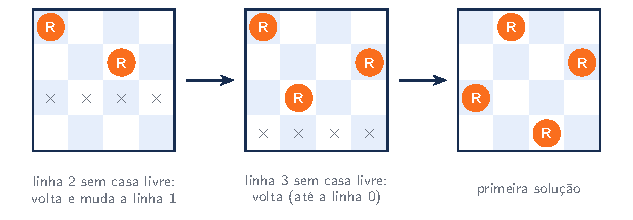
\includegraphics[width=0.85\linewidth,keepaspectratio]{imagens/capitulo-09_rainhas.pdf}
\end{center}

\begin{codigo}
\begin{Verbatim}[breaklines=true, breaksymbolleft={}, fontsize=\footnotesize]
#include <iostream>
#include <cstdlib>     // abs
using namespace std;

const int N = 8;

// a linha "linha" pode receber uma rainha na coluna "col"?
bool livre(const int coluna[], int linha, int col) {
    for (int l = 0; l < linha; l++) {
        if (coluna[l] == col) return false;     // mesma coluna
        if (abs(coluna[l] - col) == linha - l) { // mesma diagonal
            return false;
        }
    }
    return true;
}

void mostrar(const int coluna[]) {
    for (int l = 0; l < N; l++) {
        for (int c = 0; c < N; c++) {
            cout << (coluna[l] == c ? " R" : " .");
        }
        cout << endl;
    }
}

void posicionar(int coluna[], int linha, int &solucoes) {
    if (linha == N) {                   // as N rainhas estão lá
        solucoes++;
        if (solucoes == 1) mostrar(coluna); // só a primeira
        return;
    }
    for (int col = 0; col < N; col++) {
        if (livre(coluna, linha, col)) {
            coluna[linha] = col;            // escolhe e avança
            posicionar(coluna, linha + 1, solucoes);
        }        // a próxima volta do for sobrescreve a escolha
    }
}

int main() {
    int coluna[N];
    int solucoes = 0;
    posicionar(coluna, 0, solucoes);
    cout << solucoes << " soluções" << endl;   // 92 soluções
    return 0;
}
\end{Verbatim}
\end{codigo}

A primeira solução encontrada, mostrada pelo programa, é:

\begin{codigo}
\begin{Verbatim}[breaklines=true, breaksymbolleft={}, fontsize=\footnotesize]
// saída
 R . . . . . . .
 . . . . R . . .
 . . . . . . . R
 . . . . . R . .
 . . R . . . . .
 . . . . . . R .
 . R . . . . . .
 . . . R . . . .
92 soluções
\end{Verbatim}
\end{codigo}

Aqui, desfazer a escolha não exige um comando explícito: a próxima volta do laço grava outra coluna em \texttt{coluna[linha]}, e a função \texttt{livre} só olha as linhas anteriores à atual. Em vez de testar as $8^8$ (mais de 16 milhões) formas de pôr uma rainha por linha, o backtracking abandona cada tentativa assim que um conflito aparece, e a função \texttt{posicionar} é chamada apenas 2.057 vezes. Mudando \texttt{N}, o programa resolve tabuleiros de outros tamanhos: há 2 soluções para $N = 4$, 10 para $N = 5$ e 4 para $N = 6$.

\subsection{Erros Comuns}

\begin{itemize}
  \item \textbf{Esquecer o caso base.} A recursão nunca para, e o programa termina com estouro de pilha.
  \item \textbf{Não diminuir o problema.} Cada chamada recursiva precisa se aproximar do caso base; \texttt{f(n)} chamando \texttt{f(n)} é um laço infinito disfarçado.
  \item \textbf{Esquecer o \texttt{return} da chamada recursiva.} Em uma função que devolve valor, escrever \texttt{fatorial(n - 1);} sem usar o resultado joga a resposta fora.
  \item \textbf{Usar recursão que repete trabalho.} Como no Fibonacci, duas chamadas que resolvem os mesmos subproblemas fazem o tempo explodir. Use memoização ou um laço.
  \item \textbf{Recursão profunda demais.} Uma soma recursiva de um vetor com um milhão de elementos cria um milhão de registros na pilha. Para sequências longas, use um laço.
  \item \textbf{Esquecer de desfazer a escolha no backtracking.} A tentativa seguinte começa de um estado errado.
  \item \textbf{Tentar acompanhar todas as chamadas de cabeça.} Confie que a chamada recursiva resolve o problema menor e verifique só o caso base e a combinação.
\end{itemize}
